\chapter{Using Recurrent Neural Networks for Slot Filling in Spoken Language Understanding}
\label{chap:rnn}

\section{Introduction}

The term "spoken language understanding" (SLU) refers to the targeted
understanding of human speech directed at machines [1]. The goal of such
"targeted" understanding is to convert the recognition of user input, $S_i$, into
a task-specific semantic representation of the user's intention, $U_i$ at each
turn. The dialog manager then interprets $U_i$ and decides on the most
appropriate system action, $A_i$, exploiting semantic context, user specific
meta-information, such as geo-location and personal preferences, and other
contextual information.

The semantic parsing of input utterances in SLU typically consists of three
tasks: domain detection, intent determination, and slot filling. Originating
from call routing systems, the domain detection and intent determination tasks
are typically treated as semantic utterance classification problems [2,3,4,30].
Slot filling is typically treated as a sequence classification problem in which
contiguous sequences of words are assigned semantic class labels.
[5,7,31,32,33,34,40,55]. 

In this paper, following the success of deep learning methods for semantic
utterance classification such as domain detection [30] and intent determination
[13,39,50], we focus on applying deep learning methods for slot filling.
Standard approaches to solving the slot filling problem include generative
models, such as HMM/CFG composite models [31,5,53], hidden vector state (HVS)
model [33], and discriminative or conditional models such as conditional random
fields (CRFs) [6,7,32,34,40,51,54] and support vector machines (SVMs) [52].
Despite many years of research, the slot filling task in SLU is still a
challenging problem, and this has motivated the recent application of a number
of very successful continuous-space, neural net, and deep learning approaches,
e.g. [13,15,24,30,56]. 

In light of the recent success of these methods, especially the success of RNNs
in language modeling [22,23] and in some preliminary SLU experiments
[15,24,30,56], in this paper we carry out an in-depth investigation of RNNs for
the slot filling task of SLU. In this work, we implemented and compared several
important RNN architectures, including the Elman-type networks [16],
Jordan-type networks [17] and their variations. To make the results easy to
reproduce and rigorously comparable, we implemented these models using the
common Theano neural network toolkit [25] and evaluated them on the standard
ATIS (Airline Travel Information Systems) benchmark. We also compared our
results to a baseline using conditional random fields (CRF). Our results show
that on the ATIS task, both Elman-type networks and Jordan-type networks
outperform the CRF baseline substantially, and a bi-directional Jordan-type
network that takes into account both past and future dependencies among slots
works best.

In the next section, we formally define the semantic utterance
classification problem along with the slot filling task and present the
related work. In Section \ref{sec:deepreview}, we propose a brief review of deep learning
for slot filling. Section \ref{sec:rnnsf} more specifically describes our approach of
RNN architectures for slot filling. We describe sequence level
optimization and decoding methods in Section \ref{sec:slod}. Experimental results
are summarized and discussed in section \ref{sec:exp}.

\section{Slot Filling in Spoken Language Understanding}
\label{sec:sfslu}

A major task in spoken language understanding in goal-oriented human-machine
conversational understanding systems is to automatically extract semantic
concepts, or to fill in a set of arguments or "slots" embedded in a semantic
frame, in order to achieve a goal in a human-machine dialogue. 

An example sentence is provided here, with domain, intent, and slot/concept
annotations illustrated, along with typical domain-independent named entities.
This example follows the popular in/out/begin (IOB) representation, where {\it
Boston} and {\it New York} are the departure and arrival cities specified as
the slot values in the user's utterance, respectively.

TODO TABLE IOB REPRESENTATION

While the concept of using semantic frames (templates) is motivated by the case
frames of the artificial intelligence area, the slots are very specific to the
target domain and finding values of properties from automatically recognized
spoken utterances may suffer from automatic speech recognition errors and poor
modeling of natural language variability in expressing the same concept. For
these reasons, spoken language understanding researchers employed statistical
methods. These approaches include generative models such as hidden Markov
models, discriminative classification methods such as CRFs, knowledge-based
methods, and probabilistic context free grammars. A detailed survey of these
earlier approaches can be found in [7].

For the slot filling task, the input is the sentence consisting of a sequence
of words, $L$, and the output is a sequence of slot/concept IDs, $S$, one for each
word. In the statistical SLU systems, the task is often formalized as a pattern
recognition problem:  Given the word sequence $L$, the goal of SLU is to find the
semantic representation of the slot sequence $S$ that has the maximum {\it a
posteriori} probability $P(S | L)$. 

In the generative model framework, the Bayes rule is applied:

TODO EQUATION %S ̂= argmax_S P(S│L)=argmax_S P(L│S)P(S)

The objective function of a generative model is then to maximize the joint
probability $P(L | S)P(S) = P(L, S)$ given a training sample of $L$, and its semantic
annotation, $S$.

The first generative model, used by both the AT\&T CHRONUS system [31] and the
BBN Hidden Understanding Model (HUM) [35], assumes a deterministic one-to-one
correspondence between model states and the segments, i.e., there is only one
segment per state, and the order of the segments follows that of the states.  

As another extension, in the Hidden Vector State model the states in the
Markov chain representation encode all the structure information about the
tree using stacks, so the semantic tree structure (excluding words) can be
reconstructed from the hidden vector state sequence. The model imposes a hard
limit on the maximum depth of the stack, so the number of the states becomes
finite, and the prior model becomes the Markov chain in an HMM [33].

Recently, discriminative methods have become more popular. One of the most
successful approaches for slot filling is the conditional random field (CRF)
[6] and its variants. Given the input word sequence $L_1^N=l_1,\dots,l_N$, the
linear-chain CRF models the conditional probability of a concept/slot sequence
$S_1^N=s_1,\dots,s_N$ as follows:

TODO EQUATION NUM% P(S_1^N│L_1^N )=1/Z ∏_(t=1)^N▒e^(H(s_(t-1),s_t,l_(t-d)^(t+d)))             
%where EQUATION NUM 2 H(s_(t-1),s_t,l_(t-d)^(t+d) )=∑_(m=1)^M▒〖λ_m h_m (s_(t-1),s_t,l_(t-d)^(t+d))〗

and $h_m (s_{t-1},s_t,l_{t-d}^{t+d})$ are features extracted from the current and
previous states $s_t$ and $s_{t-1}$, plus a window of words around the current word
$l_t$, with a window size of $2d+1$.

CRFs have first been used for slot filling by Raymond and Riccardi [33]. CRF
models have been shown to outperform conventional generative models. Other
discriminative methods such as the semantic tuple classifier based on SVMs [36]
has the same main idea of semantic classification trees as used by the Chanel
system [37], where local probability functions are used, i.e., each phrase is
separately considered to be a slot given features. More formally,

TODO EQNUM 3 % P(S_1^N│L_1^N )=∏_(t=1)^N▒〖P(s_t |s_1^(t-1),L_1^N)〗   (3)

These methods treat the classification algorithm as a black box implementation
of linear or log-linear approaches but require good feature engineering. As
discussed in [57,13], one promising direction with deep learning architectures
is integrating both feature design and classification into the learning
procedure.

\section{Deep Learning Review}
\label{sec:deepreview}

In comparison to the above described techniques, deep learning uses many layers
of neural networks [57]. It has made strong impacts on applications ranging
from automatic speech recognition [8] to image recognition [10]. 

A distinguishing feature of NLP applications of deep learning is that inputs
are symbols from a large vocabulary, which led the initial work on neural
language modeling [26] to suggest map words to a learned distributed
representation either in the input or output layers (or both), with those
embeddings learned jointly with the task. Following this principle, a variety
of neural net architectures and training approaches have been successfully
applied [11,13,20,22,23,39,49,58,59,60,61]. Particularly, RNNs [22,23,49] are
also widely used in NLP. One can represent an input symbol as a one-hot vector,
i.e., containing zeros except for one component equal to one, and this weight
vector is considered as a low-dimensional continuous valued vector
representation of the original input, called word embedding. Critically, in
this vector space, similar words that have occurred syntactically and
semantically tend to be placed by the learning procedure close to each other,
and relationships between words are preserved. Thus, adjusting the model
parameters to increase the objective function for a training example which
involves a particular word tends to improve performances for similar words in
similar context, thereby greatly improving generalization and addressing the
curse-of-dimensionality obstacle faced with traditional n-gram non-parametric
models [26].

One way of building a deep model for slot filling is to stack several neural
network layers on top of each other. This approach was taken in [27], which
used deep belief networks (DBNs), and showed superior results to a CRF baseline
on ATIS. The DBNs were built with a stack of Restricted Boltzmann Machines
(RBMs) [12]. The RBM layers were pre-trained to initialize the weights. Then
the well-known back-propagation algorithm was used to fine-tune the weights of
the deep network in a discriminative fashion. Once the individual local models
are trained, Viterbi decoding is carried out to find the best slot sequence
given the sequence of words. 

In contrast to using DBNs, we propose recurrent neural networks (RNNs). The
basic RNNs used in language modeling read an input word and predict the next
word. For SLU, these models are modified to take a word and possibly other
features as input, and to output a slot value for each word. We will describe
RNNs in detail in the following section. 

\section{Recurrent Neural Networks for Slot-Filling}
\label{sec:rnnsf}

We provide here a description of the RNN models used for the slot filling task. 

\subsection{Words Embeddings}

The main input to a RNN is a one-hot representation of the next input word. The
first-layer weight matrix defines a vector of weights for each word, whose
dimensionality is equal to the size of the hidden layer (Fig.~\ref{fig:rnn}) - typically a
few hundred. This provides a continuous-space representation for each word.
These neural word embeddings [26] may be trained a-priori on external data such
as the Wikipedia, with a variety of models ranging from shallow neural networks
[21] to convolutional neural networks [20] and RNNs [22]. Such word embeddings
actually present interesting properties [23] and tend to cluster [20] when
their semantics are similar.

\begin{figure}[t]
\begin{center}
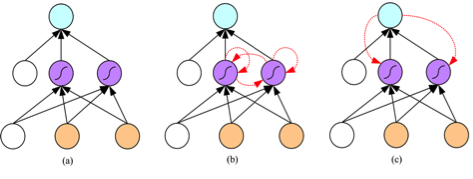
\includegraphics[width=.8\linewidth]{article4/images/rnn.png}
\caption{\label{fig:rnn} Three different types of neural networks 
(a) Feed-forward NN; (b) Elman-RNN; (c) Jordan-RNN}
\vspace{-0.2in}
\end{center}
\vspace*{-1mm}
\end{figure}


While [15][24] suggest initializing the embedding vectors with unsupervised
learned features and then fine-tune it on the task of interest, we found that
directly learning the embedding vectors initialized from random values led to
the same performance on the ATIS dataset, when using the SENNA
\footnote{http://ml.nec-labs.com/senna/} word embeddings. While this behavior
seems very specific to ATIS, we considered extensive experiments about
different unsupervised initialization techniques out of the scope of this
paper. Word embeddings were initialized randomly in our experiments.

\subsection{Context Word Window}

Before considering any temporal feedback, one can start with a context word
window as input for the model. It allows one to capture short-term temporal
dependencies given the words surrounding the word of interest. Given $d_e$ the
dimension of the word embedding and $|V|$ the size of the vocabulary, we
construct the d-context word window as the ordered concatenation of $2d+1$ word
embedding vectors, i.e. $d$ previous word followed by the word of interest and $d$
next words, with the following dot product:

TODO EQ NON NUMEROTE %C_d (l_(i-d)^(i+d) )=E ̃l ̃_(i-d)^(i+d)∈R^(d_e (2d+1))

where $\tilde{E}$ corresponds to the embedding matrix
$E\in\mathcal{M}_{d_e\times|V|}(\mathbb{R})$ replicated vertically $2d+1$ times
and $\tilde{l}_{i-d}^{i+d}= [
\tilde{l}_{i-d},\dots,\tilde{l}_i,\dots,\tilde{l}_{i+d}]^T\in\mathbb{R}^{|V|(2d+1)}$
corresponds to the concatenation of one-hot word index vectors $\tilde{l}_i$.

TODO FIGURE ONEHOT

In this window approach, one might wonder how to build a $d$-context window for
the first/last words of the sentence. We work around this border effect problem
by padding the beginning and the end of sentences $d$ times with a special token.
Below, we depict an example of building a context window of size $3$ around the
word "from":

TODO FIGURE

In this example, $l(t)$ is a $3$-word context window around the $t$-th word
"from".  $l_{\textrm{from}}$ corresponds to the appropriate line in the
embedding matrix $E$ mapping the word "from" to its word embedding. Finally,
$C_3 (t)$ gives the ordered concatenated word embeddings vector for the
sequence of words in $l(t)$.

\subsection{Elman, Jordan and Hybrid architectures}

As in [15], we describe here the two most common RNN architectures in the
literature: the Elman [16] and Jordan [17] models. The architectures of these
models are illustrated in Fig.~\ref{fig:rnn}.

In contrast with classic feed-forward neural networks, the Elman neural network
keeps track of the previous hidden layer states through its recurrent
connections. Hence, the hidden layer at time $t$ can be viewed as a state
summarizing past inputs along with the current input. Mathematically, Elman
dynamics with $d_h$ hidden nodes at each of the $H$ hidden layers are depicted
below:

TODO EQUATIONS NUM 4 5

where we used the non-linear sigmoid function applied element wise for the
hidden layer $f(x)=1/(1+\exp^(-x))$ and $h^{(i)} (0)\in\mathbb{R}^{d_h}$ are parameter vectors
to be learned. The superscript denotes the depth of the hidden layers and $U^{'}$
represents the recurrent weights connection. The posterior probabilities of the
classifier for each class are then given by the softmax function applied to the
hidden state:

TODO EQUATIONS NUM 6

Where $V$ correspond to the weights of the softmax top layer. 

The learning part then consists of tuning the parameters $\theta=\{ E, h^{(1)}
(0), U^{(1)}, \\ U^{'(1)},\dots,h^{(H)} (0), U^{(H)}, U^{'(H)} ,V \}$   of the RNN with $N$
output classes. Precisely, the matrix shapes are $U^{(1)}\in\mathcal{M}_{d_h\times d_e (2d+1)}
(\mathbb{R})$~;~ $U^{'(1)},\dots,U^{(H)}, U^{'(H)}\in\mathcal{M}_{d_h\times d_h} (\mathbb{R})$ and $V\in\mathcal{M}_{N\times d_h}(\mathbb{R})$. For
training, we use stochastic gradient descent, with the parameters being updated
after computing the gradient for each one of the sentences in our training set
$\mathcal{D}$, towards minimizing the negative log-likelihood. Note that a sentence is
considered as a tuple of words and a tuple of slots:

TODO EQ NUM 7

Note that the length $T$ of each sentence can vary among the training samples and
the context word window size $d$ is a hyper-parameter.  

The Jordan RNN is similar to the Elman-type network except that the recurrent
connections take their input from the output posterior probabilities:

TODO EQ NUM 8

where $U^{'}\in\mathcal{M}_{d_h\times N} (\mathbb{R})$ and
TODO %$Ρ(y(0))\in\mathbb{R}^N$ are additional parameters to tune. As pointed out in
[15], three different options can be considered for the feedback connections:
TODO %(a) $Ρ(y(t-1))$, (b) a one-hot vector with an active bit for $\textrm{arg} \max_i⁡P_i
%(y(t-1))$ or even (c) the ground truth label for training.  Empirically [15],
none of these options significantly outperformed all others.  

In this work, we focused on the Elman-type, Jordan-type and hybrid versions of
RNNs. The hybrid version corresponds to a combination of the recurrences from
the Jordan and the Elman models:

TODO EQ

\subsection{Forward, Backward and Bidirectionnal variants}

In slot filling, useful information can be extracted from the future and we do
not necessarily have to process the sequence online in a single forward pass.
It is also possible to take into account future information with a single
backward pass but still, this approach uses only partial information available.
A more appealing model would consider both past and future information at the
same time: it corresponds to the bi-directional Elman [18][19] or Jordan [15]
RNN.




\section{Sequence Level Optimization and Decoding} \label{sec:slod}

\section{Experimental Results}
\label{sec:exp}

\section{Conclusions}
\label{sec:conclu}
